\subsection{Na\"{i}ve Approach}
We consider model parallelizing the training of a DNN on a distributed-memory 
system using MPI. Figure~\ref{fig:altsplit_baseline} illustrates a na\"{i}ve 
approach to it which also serves as the baseline of this chapter. It depicts a 
5-layer all-connected DNN split on two MPI processes and the 4 neurons per layer 
are evenly assigned to each MPI process. The input and output layer are omitted 
and we assume they are replicated in every MPI process. The black arrows in the 
figure indicate all-to-all communications between the two MPI processes. During 
both the forward- and backward-propagation, each neuron from the current layer 
needs the outputs of the entire neurons from the preceding layer. All-to-all 
communication will have to happen across all the MPI processes. In the figure, 
prior to the computation of each layer 4 all-to-all communication need to occur 
so that the output information from the preceding layer can get to be fully 
propagated to the respective portions of the current layer to all the MPI 
processes.  Albeit some numerical rounding errors introduced due to the 
non-deterministic nature of the all-to-all communication, this approach 
guarantees that the output information from the preceding layer is consistent 
and identical across all the MPI processes prior to the computation of their 
respective portions of the current layer.
\begin{figure}[H]
    \centerline{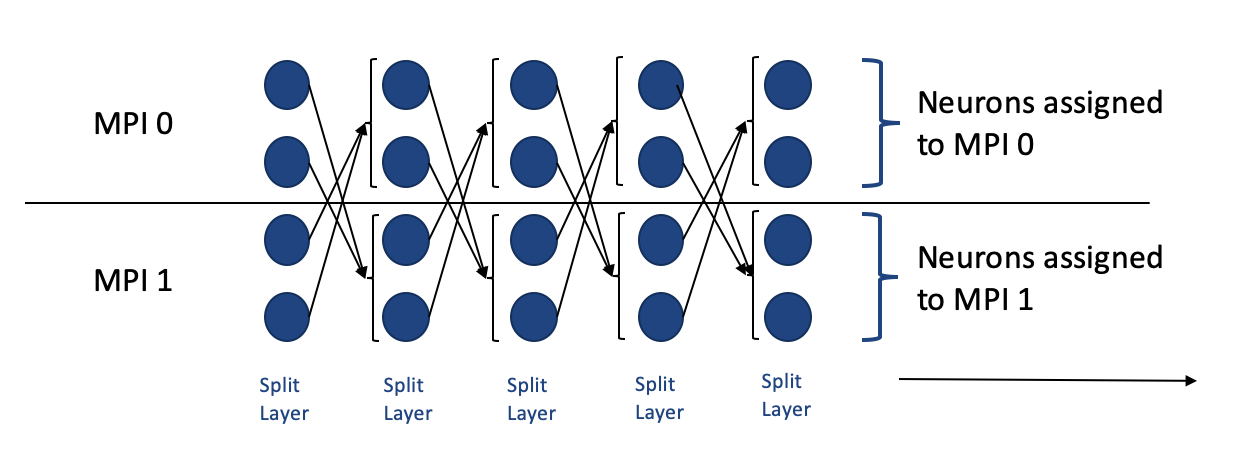
\includegraphics[scale=0.60]{altsplit/figs/baseline.png}}
    \caption{Baseline model parallelism scheme}
    \label{fig:altsplit_baseline}
\end{figure}

%We show the differences between sequential and the baseline modell parallel 
%training of DNN side by side in Algorithm~\ref{alg:altsplit_sequential} and 
%\ref{alg:altsplit_baseline}.
The sequential training of a DNN using matrix operations is shown in 
Algorithm~\ref{alg:altsplit_sequential}. We denote $bs$ as the batch size, $L$ 
as the number of layers, $N$ as the number of neurons in one layer. Matrix is 
denoted as $\pmb{A}[m,n]$ whereas $m$ and $n$ stand for the number of rows and 
columns respectively of the matrix. $\phi$ is an element-wise non-linear 
function (tanh, relu etc.).
\begin{algorithm}[H]%algorithm* occupies full page
\caption{Sequential DNN}
\label{alg:altsplit_sequential}
{\fontsize{10}{10}\selectfont
\begin{algorithmic}[1]
    \For {$l = 1 \ldots L$}
    \Comment Fowardpropagation 
        \State $\pmb{Y}_l[bs, N_l] = \pmb{O}_{l-1}[bs, N_{l-1}] * \pmb{W}_{l}[N_{l-1}, N_l]$
        \State $\pmb{O}_l[bs, N_l] = \phi(\pmb{Y}[bs, N_l])$
    \EndFor
    \For {$l = L \ldots 1$}
    \Comment Backpropagation 
    \State $\nabla \pmb{W}_l[bs, N_l]  = \nabla \pmb{W}_{l+1}[bs, N_{l+1}] * \pmb{W}_{l+1}[N_l, N_{l+1}]$
    \State $\nabla \pmb{W}_l[bs, N_l] = \nabla \pmb{W}_l[bs, N_l] * (\partial \pmb{O}_l[bs, N_l] / \partial \pmb{Y}_l[bs, N_l]$)
    \EndFor
    \State Update parameters
\end{algorithmic}}
\end{algorithm}

\begin{algorithm}[H]
\caption{Na\"{i}ve model parallelism of DNN}
\label{alg:altsplit_baseline}
{\fontsize{10}{10}\selectfont
\begin{algorithmic}[1]
    \ForAll {$p \in MPI\_Processes$}
    \Comment Fowardpropagation 
        \For {$l = 1 \ldots L$}
            \State MPI\_Allgather on $\pmb{O}_{l-1}[bs, N_{l-1}$
            %\State All-to-All communication
            \State $\pmb{Y}_l[bs, N_l] = \pmb{O}_{l-1}[bs, N_{l-1}] * \pmb{W}_{l}[N_{l-1}, N_l]$
            \State $\pmb{O}_l[bs, N_l] = \phi(\pmb{Y}[bs, N_l])$
        \EndFor
    \EndFor
    \ForAll {$p \in MPI\_Processes$}
    \Comment Backpropagation 
        \For {$l = 1 \ldots L$}
            \State All-to-All communication
            \State $\nabla \pmb{W}_l[bs, N_l]  = \nabla \pmb{W}_{l+1}[bs, N_{l+1}] * \pmb{W}_{l+1}[N_l, N_{l+1}]$
            \State $\nabla \pmb{W}_l[bs, N_l] = \nabla \pmb{W}_l[bs, N_l] * (\partial \pmb{O}_l[bs, N_l] / \partial \pmb{Y}_l[bs, N_l]$)
        \EndFor
    \EndFor
    \ForAll {$p \in MPI\_Processes$}
        \State Update parameters
    \EndFor
\end{algorithmic}}
\end{algorithm}

\subsection{Altsplit (Alternate Split) Approach}
We propose the \emph{Altsplit} approach which splits or replicates the layers 
alternately. The scheme is illustrated in Figure~\ref{fig:altsplit_scheme} with 
the same 5-layer DNN as in Figure~\ref{fig:altsplit_baseline}. The first layer 
is split across MPI processes whereas the next layer is replicated over 
the MPI processes with the same initialization values. Subsequent layers are 
constructed with alternating splits and replications.

As in the na\"{i}ve approach, all-to-all communication has to happen if the 
preceding layer is split over the MPI processes. In order to 

\begin{figure}[H]
    \centerline{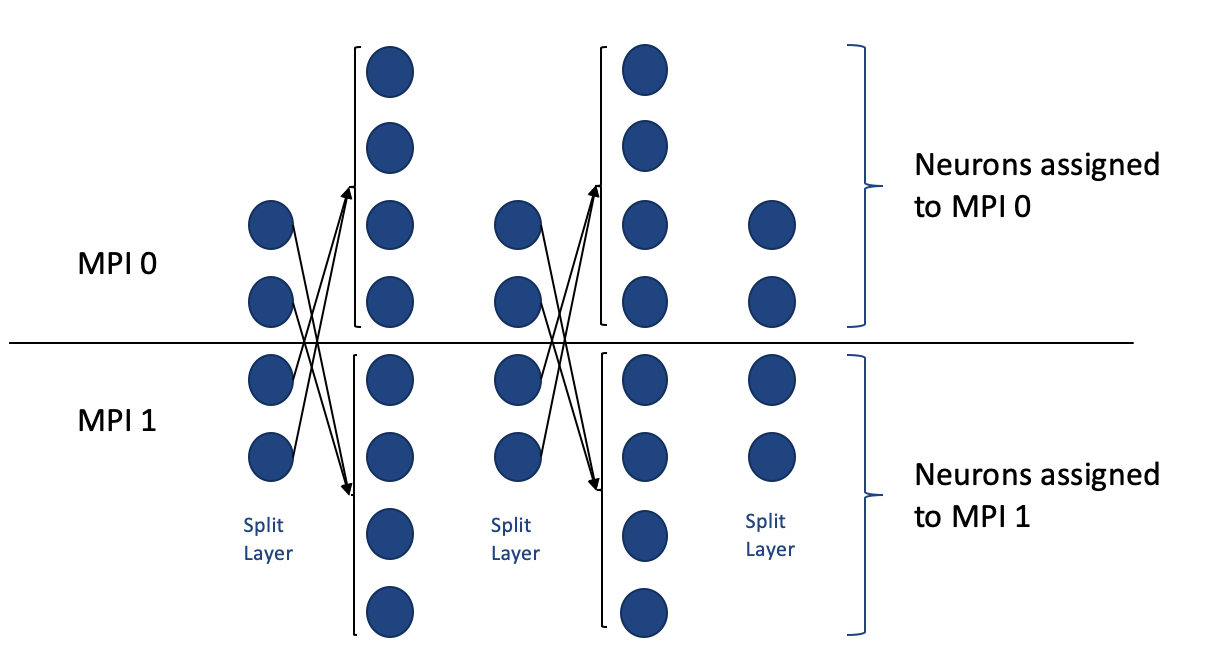
\includegraphics[scale=0.60]{altsplit/figs/altsplit.png}}
    \caption{The \emph{Altsplit} scheme}
    \label{fig:altsplit_scheme}
\end{figure}
